

\section{Exploración Univariada}\label{univariada}

En esta sección exploro cada índice. En esta sección exploro cada índice. En esta sección exploro cada índice. En esta sección exploro cada índice. En esta sección exploro cada índice. En esta sección exploro cada índice. En esta sección exploro cada índice. En esta sección exploro cada índice. En esta sección exploro cada índice.

% Table created by stargazer v.5.2.2 by Marek Hlavac, Harvard University. E-mail: hlavac at fas.harvard.edu
% Date and time: vie., jun. 29, 2018 - 7:29:37 p.m.
\begin{table}[!htbp] \centering 
  \caption{Medidas estadísticas} 
  \label{stats} 
\begin{tabular}{@{\extracolsep{5pt}}lccccccc} 
\\[-1.8ex]\hline 
\hline \\[-1.8ex] 
Statistic & \multicolumn{1}{c}{N} & \multicolumn{1}{c}{Mean} & \multicolumn{1}{c}{St. Dev.} & \multicolumn{1}{c}{Min} & \multicolumn{1}{c}{Pctl(25)} & \multicolumn{1}{c}{Pctl(75)} & \multicolumn{1}{c}{Max} \\ 
\hline \\[-1.8ex] 
IDH & 32 & 0.802 & 0.042 & 0.691 & 0.768 & 0.834 & 0.879 \\ 
Poblacion.Cabecera & 32 & 1,196,730.000 & 1,982,287.000 & 13,090 & 234,624.2 & 970,925.2 & 10,070,801 \\ 
Poblacion.Resto & 32 & 360,590.300 & 331,887.600 & 21,926 & 96,968.8 & 487,529.5 & 1,428,858 \\ 
Poblacion.Total & 32 & 1,557,320.000 & 2,202,522.000 & 43,446 & 371,160.8 & 1,512,087 & 10,985,285 \\ 
\hline \\[-1.8ex] 
\end{tabular} 
\end{table} 
\begin{figure}[h]
\centering
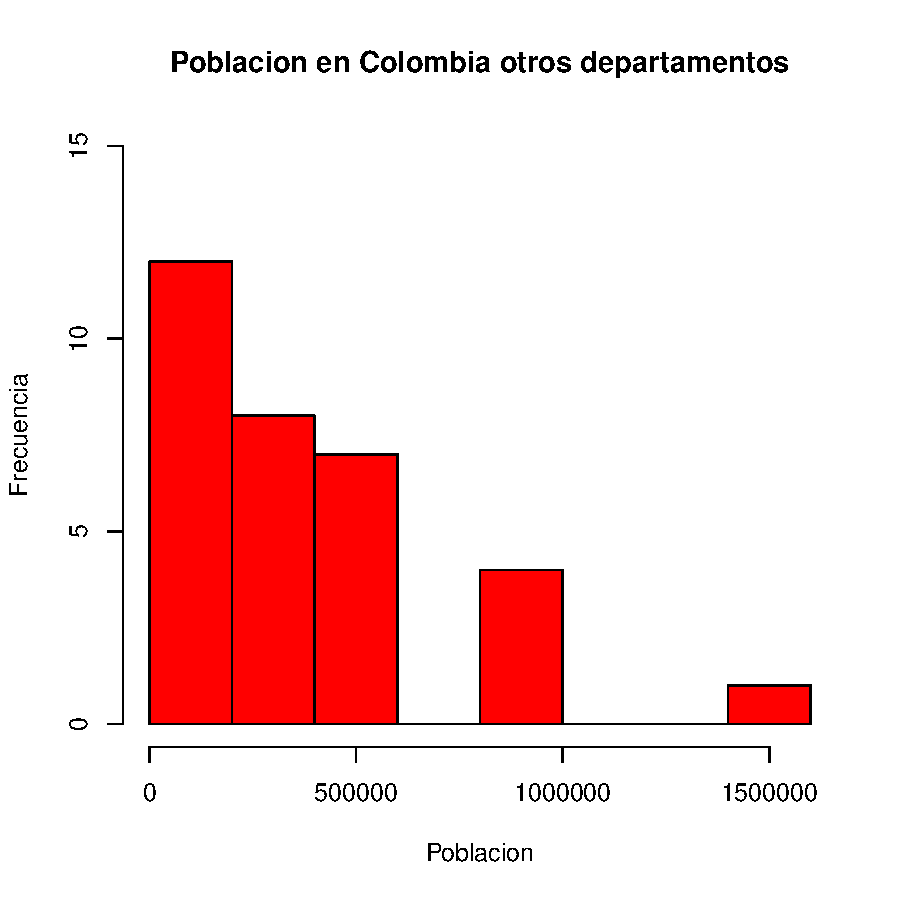
\includegraphics{univariada-summaryDatos}
\caption{Histograma del IDH en Colombia para los 32 departamentos}
\label{barplot1}
\end{figure}

\begin{figure}[h]
\centering
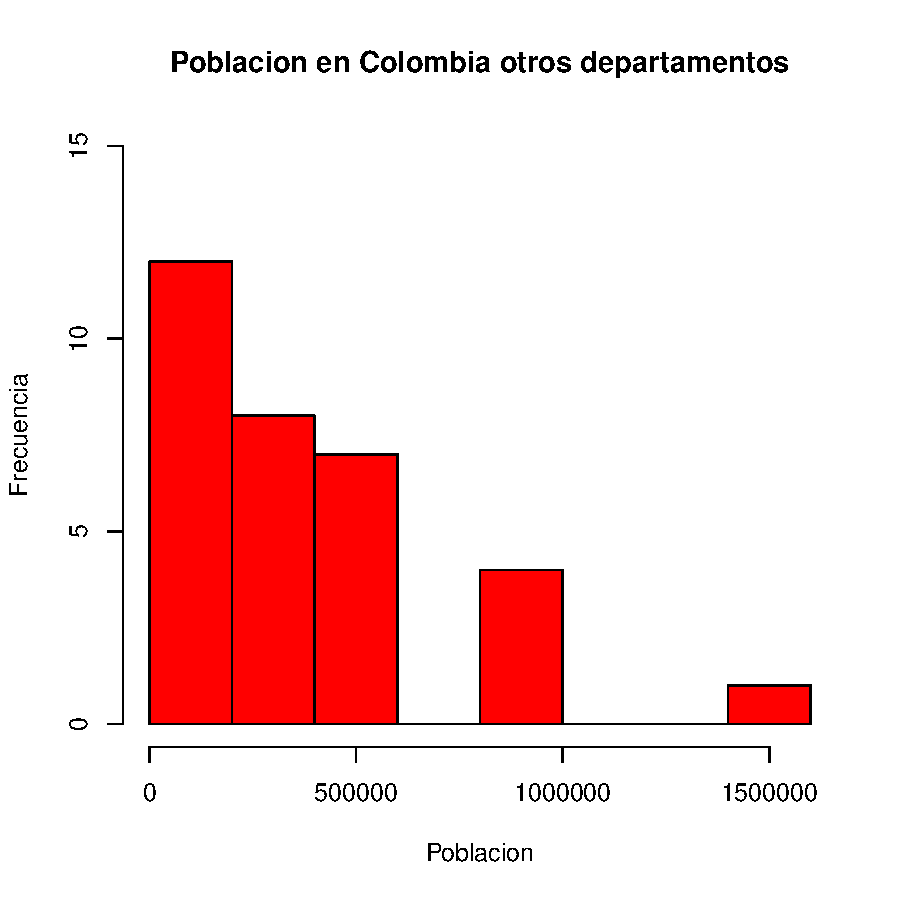
\includegraphics{univariada-summaryDatos}
\caption{Histograma de la poblacion en Colombia para los departamentos de cabecera}
\label{barplot2}
\end{figure}
\begin{figure}[h]
\centering
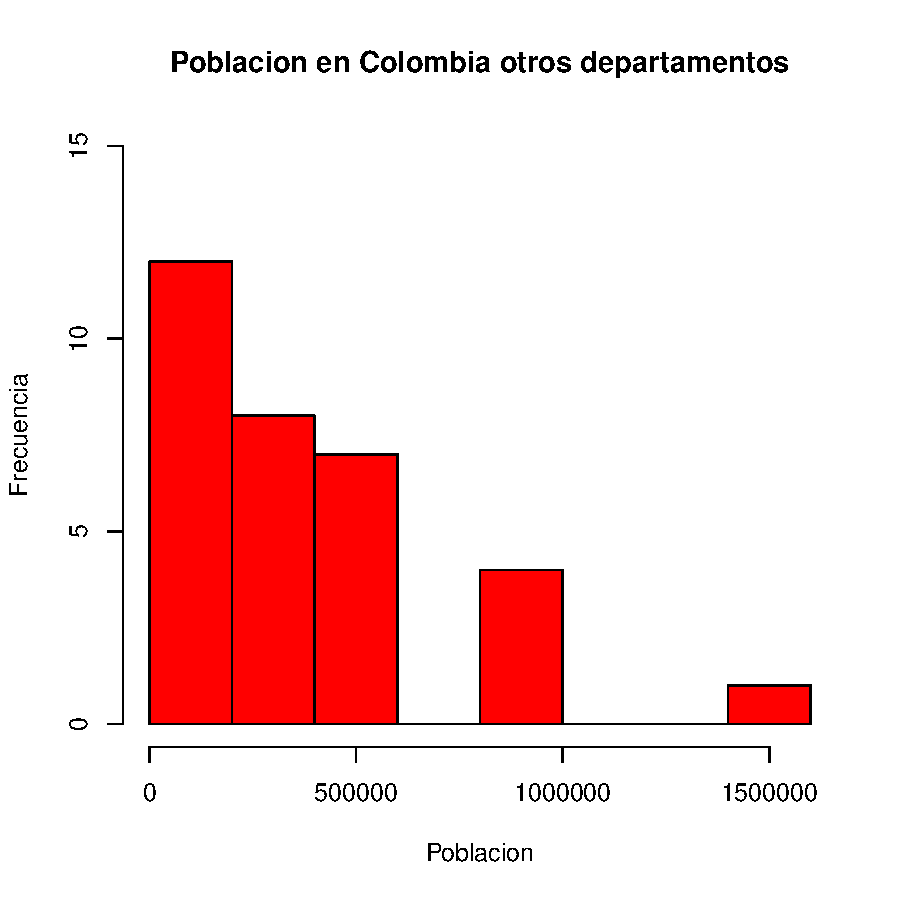
\includegraphics{univariada-summaryDatos}
\caption{Histograma de la poblacion en Colombia para los otros departamentos}
\label{barplot3}
\end{figure}
Para conocer el comportamiento de las variables se ha preparado la Tabla %\ref{Tfrecuencias}, donde se describe la distribución de las modalidades de cada variable. Los números representan la situación de algun país en ese indicador, donde el mayor valor numérico es la mejor situación.
\begin{figure}[h]
\centering
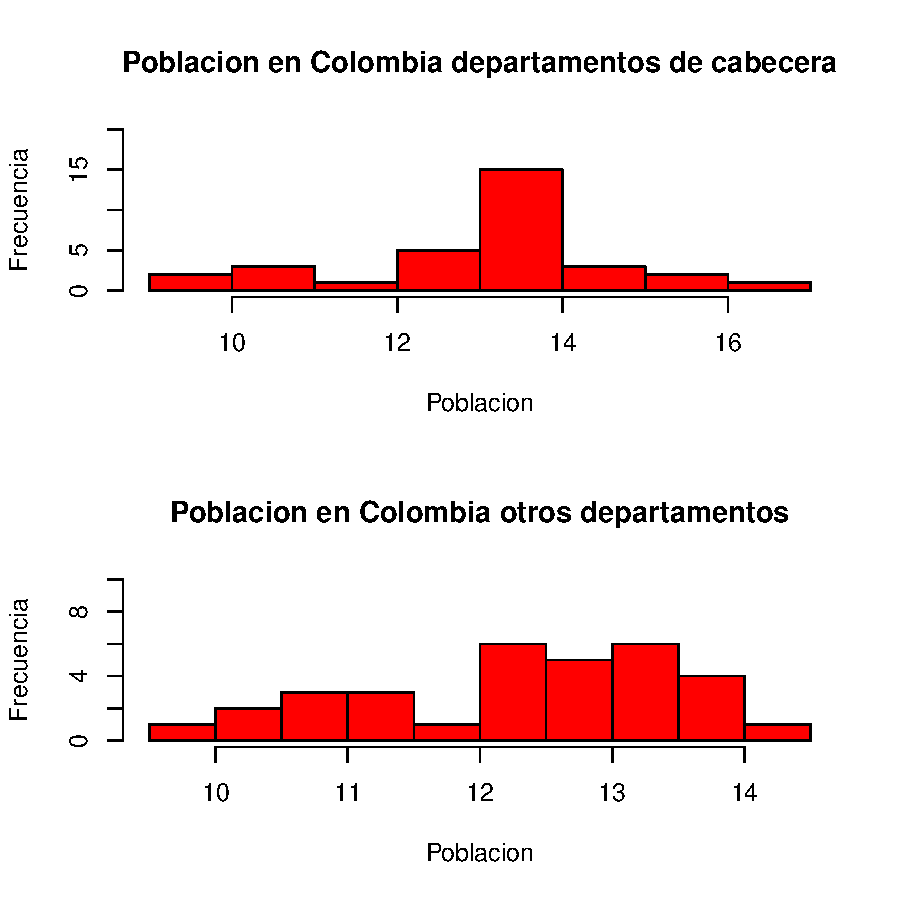
\includegraphics{univariada-rehacerhistogramas}
\caption{Histograma transformado de la poblacion en Colombia para los 32 departamentos}
\label{barplot4}
\end{figure}
